% \paragraph{Western Bias in Wikidata.}
\paragraph{Regional Knowledge Gap: Western vs. Non-Western Representation.}
Regional knowledge gap analysis in Wikidata will be performed on 5 Wikidata classes: computer scientist, singer, memorial, university, and river. For each class, we collected the data for the western portion from 8 countries: Canada, France, Germany, Ireland, Poland, Switzerland, the United Kingdom (UK), and the United State of America (USA). For the non-western portion, we also selected 8 countries: China, Egypt, India, Indonesia, Japan, Morocco, Nigeria, and South Africa. The selected countries represent different continents to capture a diverse geographic distribution. Additionally, we focused on large and well-known countries to ensure the dataset is representative, as data from smaller countries may not provide meaningful insights due to limited coverage in Wikidata.

To analyze the gap, the first aspect that will be considered is the proportion of each regional category in every class. We assumed that there are equal numbers of western and non-western and this will be the basis to determine if there is any gap in the data. Pearson's chi-square test (goodness-of-fit) is then performed to test the null and alternative hypotheses with significance level of \(\alpha=5\%\) as follows:

% \(H_0\): The proportions of western and non-western entities in a particular class are equal

% \(H_1\): The proportions of western and non-western entities in a particular class are not equal

\begin{table}[h]
    \centering
    \renewcommand{\arraystretch}{1.3}
    \begin{tabular}{|l p{12cm}|} 
        \hline
        \multicolumn{2}{|l|}{\textbf{Regional Knowledge Gap: Entity Count Gap (Pearson's chi-square test)}} \\
        \hline
        \textbf{$H_0$} & The proportions of western and non-western entities in a particular class are equal. \\
        \textbf{$H_1$} & The proportions of western and non-western entities in a particular class are not equal. \\
        \hline
        \textbf{Insight 1:} & Across all 5 classes, the proportions of western and non-western entities differ significantly. Western entities dominate in 4 out of 5 classes, with the only exception being the university class, which is skewed toward non-western entities. \\
        \hline
    \end{tabular}
\end{table}

% \vspace{-3em}

\begin{center}
\scriptsize
\begin{threeparttable}
\captionsetup{font=small}
\caption{Entity Count of 5 Wikidata Classes per Regional Category}
\label{tab:western - entity count}
\begin{tabular}{c | c c c c c c c} 

\toprule
    Class Name & Entity & Western & \CellWithForceBreak{Non- \\ western} & \%Western & \CellWithForceBreak{\%Non- \\ western}& $\chi^2$ & p-value \\ [0.5ex] 
\midrule
    Computer scientist & 6063 & 5446 & 617 & 0.90 & 0.10 & 3846.15 & 0.0 \\
    Singer & 43240 & 31039 & 12201 & 0.72 & 0.28 & 8206.99 & 0.0 \\
    Memorial & 4011 & 3836 & 175 & 0.96 & 0.04 & 3341.54 & 0.0 \\
    University & 6124 & 2398 & 3726 & 0.39 & 0.61 & 287.98 & 1.37e-64 \\
    River & 125567 & 70059 & 55508 & 0.56 & 0.44 & 1686.20 & 0.0 \\
    [1ex]
\bottomrule
\end{tabular}
\begin{tablenotes}
    \scriptsize
    \item{This table shows the entity count of 5 Wikidata classes per regional category. Chi-square test result shows the significance of difference between the entity count of the two regions.}
\end{tablenotes}
\end{threeparttable}
\end{center}

From \autoref{tab:western - entity count}, we can observe that the proportion of western entities exceeds that of non-western entities in 4 out of the 5 classes. In the memorial and computer scientist classes, the gap is particularly striking, with western entities making up over 90\% of the total population. Similarly, in the singer and river classes, western entities also represent the majority. The university class is the only exception, where non-western entities slightly outnumber western ones, comprising 61\% of the total. Based on the results of the chi-square test, the p-values in all five classes are well below the significance threshold ($\alpha = 0.05$), leading us to reject the null hypothesis. This indicates that the differences in entity proportions between western and non-western entities are statistically significant and not due to random variation.

However, similar to entity count in gender-based knowledg gap analysis, it is debatable that some of these gaps are expected. For instance, the dominance of western representation in the computer scientist or memorial classes is not necessarily a result of data entry errors or systemic bias within Wikidata alone. Instead, it may mirror general historical and sociopolitical factors, such as unequal access to documentation, global academic visibility, and archival infrastructure. Conversely, the university class, where the number of non-western entities are higher, might be a reflection of population-driven realities, as countries like China, India, and Indonesia possess massive populations and have established a vast number of higher education institutions to serve their demographic needs. The greater number of non-western universities represented in Wikidata is probably a result of this population scale. Due to this, raw entity count alone may not be an ideal measure of gap. To more accurately assess representation and equity, we must consider other metrics that analyze wealth distribution and prominence at the entity level.

% From \autoref{tab:western - central tendency}, non-western entities generally have lower values of measure of central tendency (mean, median, mode). The range of property count of non-westerns is generally also lower than the westerns. Positive values of skewness (skewness > 0) and high kurtosis values (kurtosis > 3) in all classes denote the wealth distribution is right skewed and leptokurtic.

The next step in our analysis is examining the measures of central tendency and dispersion to evaluate where the knowledge wealth is concentrated and how it varies between western and non-western entities.

\begin{table}[h]
    \centering
    \renewcommand{\arraystretch}{1.3}
    \begin{tabular}{|l p{12cm}|} 
        \hline
        \multicolumn{2}{|l|}{\textbf{Regional Knowledge Gap: Measures of Central Tendency and Dispersion}} \\
        \hline
        \textbf{Insight 1:} & In 4 out of 5 classes, western entities have higher mean, median, and mode values than non-western entities, indicating greater concentration of knowledge wealth. \\
        \textbf{Insight 2:} & Western entities generally exhibit higher standard deviations, skewness, and kurtosis, suggesting greater variability, more frequent outliers, and stronger right-skewed distributions. \\
        \hline
    \end{tabular}
\end{table}

% \vspace{-3em}

\begin{center}
\scriptsize
\begin{threeparttable}
\captionsetup{font=small}
\caption{Measures of Central Tendency of 5 Wikidata Classes per Regional Category}
\label{tab:western - central tendency}
\begin{tabular}{c | c c c} 
\toprule
    Class Name & \CellWithForceBreak{Mean \\ (o/w/n)} & \CellWithForceBreak{Median \\ (o/w/n)} & \CellWithForceBreak{Mode \\ (o/w/n)} \\ [0.5ex] 
\midrule
    Computer scientist & 35.00/35.87/27.24 & 29.00/29.00/22.00 & 21/15/16 \\
    Singer & 34.99/39.14/24.43 & 25.00/29.00/18.00 & 15/18/14 \\
    Memorial & 11.04/11.04/11.13 & 9.00/9.00/9.00 & 9/9/9 \\
    University & 23.11/31.61/17.63 & 17.50/24.00/16.00 & 6/6/6 \\
    River & 7.69/8.55/6.60 & 7.00/7.00/6.00 & 7/7/7 \\
    [1ex]
\bottomrule
\end{tabular}
\begin{tablenotes}
    \scriptsize
    \item{This table shows the measures of central tendency of 5 Wikidata classes per regional category. Each measure will have 3 values: o (overall), w (western), and n (non-western).}
\end{tablenotes}
\end{threeparttable}
\end{center}

% \vspace{-2em}

\begin{center}
\scriptsize
\begin{threeparttable}
\captionsetup{font=small}
\caption{Measures of Dispersion and Symmetry of 5 Wikidata Classes per Regional Category}
\label{tab:western - dispersion and symmetry}
\begin{tabular}{c | c c c c c} 

\toprule
    Class Name & \CellWithForceBreak{Min \\ (o/w/n)} & \CellWithForceBreak{Max \\ (o/w/n)} & \CellWithForceBreak{Std. Deviation \\ (o/w/n)} & \CellWithForceBreak{Skewness \\ (o/w/n)} & \CellWithForceBreak{Kurtosis \\ (o/w/n)} \\ [0.5ex] 
\midrule
    Computer scientist & 4/4/5 & 441/441/145 & 25.15/25.67/18.15 & 3.02/3.02/2.37 & 20.90/20.83/8.49 \\
    Singer & 3/4/3 & 687/687/379 & 33.27/36.60/18.94 & 4.49/4.28/3.15 & 35.56/31.09/21.59 \\
    Memorial & 2/3/2 & 142/142/52 & 5.89/5.82/7.28 & 8.50/8.95/2.98 & 143.57/156.15/12.79 \\
    University & 2/2/2 & 234/234/166 & 20.00/25.88/12.25 & 2.37/1.65/2.22 & 10.34/5.33/12.70 \\
    River & 2/2/2 & 452/452/148 & 5.24/6.46/2.68 & 21.71/19.54/14.67 & 1152.84/868.56/465.42 \\
    [1ex]
\bottomrule
\end{tabular}
\begin{tablenotes}
    \scriptsize
    \item{This table shows the measures of dispersion and symmetry of 5 Wikidata classes per regional category. Each measure will have 3 values: o (overall), w (western), and n (non-western).}
\end{tablenotes}
\end{threeparttable}
\end{center}

From \autoref{tab:western - central tendency}, we observed that in 4 out of 5 classes, western entities consistently show higher values across all measures of central tendency (mean, median, and mode) compared to non-western entities. This suggests that western entities tend to be richer in knowledge wealth. The memorial class is the only exception, where both groups exhibit nearly identical values. A particularly extreme disparity is observed in the university class, where the mean property count for western entities (31.61) is nearly double that of non-western entities (17.63), highlighting a strong central tendency skew. This extreme pattern can also be seen in the singer class.

Turning to the measures of dispersion and symmetry in \autoref{tab:western - dispersion and symmetry}, we saw that standard deviation is generally higher for western entities across all classes except memorial, suggesting greater wealth variability among western entities. Furthermore, in the university class, western entities show a standard deviation of 25.88, more than double that of non-western entities at 12.25. We also observed positive skewness and high kurtosis across all classes and both regions, indicating that knowledge wealth distributions are right-skewed and leptokurtic. However, western entities often exhibit higher values, implying more extreme outliers and longer tails. For example, in the river class, the skewness and kurtosis for western entities are 19.54 and 868.56, respectively, compared to 14.67 and 465.42 for non-western entities.

Taken together, these statistics suggest that western entities tend not only to accumulate more knowledge wealth on average but also to dominate the extreme high end of the distribution. In contrast, non-western entities tend to cluster around lower values with tighter distribution, reinforcing regional disparity in knowledge representation.

At a glance, western entities appear to be richer compared to their non-western counterparts. To statistically verify this, we conducted a series of mean comparison tests between the two groups. We began by applying the F-test to assess whether the western and non-western subsets within each class have equal variance. The result of the F-test determines the appropriate test to be used: if the p-value is greater than 0.05, indicating equal variance, we use the standard t-test; otherwise, we apply Welch's test, which does not assume equal variance.

% Out of 5 classes, class of memorial is the only class where the null hypothesis is not rejected. In the other 4 classes, we can see a significant difference between the mean of the two reginal categories, which all are in favor of the western.

\begin{table}[h!]
    \centering
    \renewcommand{\arraystretch}{1.3}
    \begin{tabular}{|l p{12cm}|} 
        \hline
        \multicolumn{2}{|l|}{\textbf{Regional Knowledge Gap: Mean of Wealth Gap (two-sided t-test and Welch's test)}} \\
        \hline
        \textbf{$H_0$} & The means of wealth of western and non-western entities in a particular class are equal. \\
        \textbf{$H_1$} & The means of wealth of western and non-western entities in a particular class are not equal. \\
        \hline
        \textbf{Insight 1:} & In 4 out of 5 classes, western entities have significantly higher mean knowledge wealth than non-western entities. \\
        \hline
    \end{tabular}
\end{table}

% \vspace{-3em}

\begin{center}
\scriptsize
\begin{threeparttable}
\captionsetup{font=small}
\caption{F-Test, T-Test, and Welch's Test Result of 5 Wikidata Classes}
\label{tab:western - mean test}
\begin{tabular}{c | c c c c c c} 
\toprule
    Class Name & \CellWithForceBreak{F-Test \\ statistic} & \CellWithForceBreak{F-Test \\ p-value} & \CellWithForceBreak{T-Test \\ statistic} & \CellWithForceBreak{T-Test \\ p-value} & \CellWithForceBreak{Welch's Test \\ statistic} & \CellWithForceBreak{Welch's \\ p-value} \\ [0.5ex] 
\midrule
    Computer scientist & 2.00 & 1.00 & 8.13 & 5.10e-16 & - & - \\
    Singer & 3.73 & 1.00 & 42.22 & 0.0 & - & - \\
    Memorial & 0.64 & 0.00 & - & - & -0.16 & 0.88 \\
    University & 4.46 & 1.00 & 28.40 & 8.23e-167 & - & - \\
    River & 5.83 & 1.00 & 66.91 & 0.0 & - & - \\
 [1ex]
\bottomrule
\end{tabular}
\begin{tablenotes}
    \scriptsize
    \item{}
\end{tablenotes}
\end{threeparttable}
\end{center}

The result of the F-test in \autoref{tab:western - mean test} shows that only one class, that is, memorial, has unequal variance (p < 0.05), thus requiring the use of Welch's test. For the remaining four classes, the t-test was applied. From the test results, we rejected the null hypothesis in 4 out of 5 classes, indicating that the difference in mean wealth between western and non-western entities is statistically significant. The only exception is the memorial class, where Welch's test yields a p-value of 0.88, suggesting no significant difference in mean. Among the classes with significant results, the direction of difference consistently favors Western entities. This can be seen clearly in classes such as university and singer, where the t-statistics are noticeably high (28.40 and 42.22, respectively) and the p-values are zero. These findings align with our previous observations that western entities dominate in terms of quantity and average information richness. We conclude that western entities are more likely to have higher mean knowledge wealth than non-western ones, although exceptions like the memorial class suggest that certain domains may present a more balanced knowledge distribution.

As with gender-based knowledge gap, measuring regional gap in Wikidata cannot rely solely on entity counts. The number of entities associated with western and non-western regions may reflect real-world disparities in documentation or notability, making raw counts an unreliable indicator of gap. Similarly, measures of central tendency, such as the mean or median, fail to capture how representation is distributed across the full spectrum of prominence or wealth. To address these limitations, we applied the same metric introduced in the gender-based gap analysis: the relative expectation ratio. This measure compares a region's share of entities within a given quantile to its expected share under equal representation. A ratio of 1 indicates proportional representation, while values above or below 1 signal overrepresentation or underrepresentation, respectively. This allows for a more nuanced, quantile-level understanding of how western and non-western entities are distributed in knowledge graphs like Wikidata.

\begin{table}[h]
    \centering
    \renewcommand{\arraystretch}{1.3}
    \begin{tabular}{|l p{12cm}|} 
        \hline
        \multicolumn{2}{|l|}{\textbf{Regional Knowledge Gap: Relative Expectation Ratios}} \\
        \hline
        \textbf{Insight 1:} & On average across all 5 classes, the less prominent segments are dominated by non-western entities, while the more prominent ones are dominated by western entities. The middle quantiles exhibit a zig-zag pattern, reflecting inconsistent representation between the two groups. \\
        \textbf{Insight 2:} & At the individual class level, 2 out of 5 classes display a particularly strong western dominance. The rests exhibit a zig-zag trend. \\
        \hline
    \end{tabular}
\end{table}

On average across all classes, the lower four quantiles (i.e., the less prominent or "poorer" segments) are predominantly composed of non-western entities, while the top three quantiles (i.e., the more prominent or "wealthier" segments) are dominated by western entities. The middle quantiles exhibit a zig-zag pattern, reflecting inconsistent representation between the two groups. At the individual class level, the computer scientist and singer classes display a particularly strong western bias. In both classes, non-western entities are consistently overrepresented in the lower quantiles (Q1–Q4), while western entities are consistently overrepresented in the upper quantiles (Q5–Q6). This pattern suggests a clear stratification, with non-western entities disproportionately concentrated in less prominent positions. The memorial, university, and river classes, however, deviate from this pattern and exhibit a zig-zag trend across quantiles. This suggests a more unstable distribution of western and non-western entities across the quantiles.

\begin{figure}
\centering 
\subfloat[Ratio of Class Wealth to Expectation per Cumulative Top Percentage - All Classes Average
\label{fig:test1 - western}]{%
  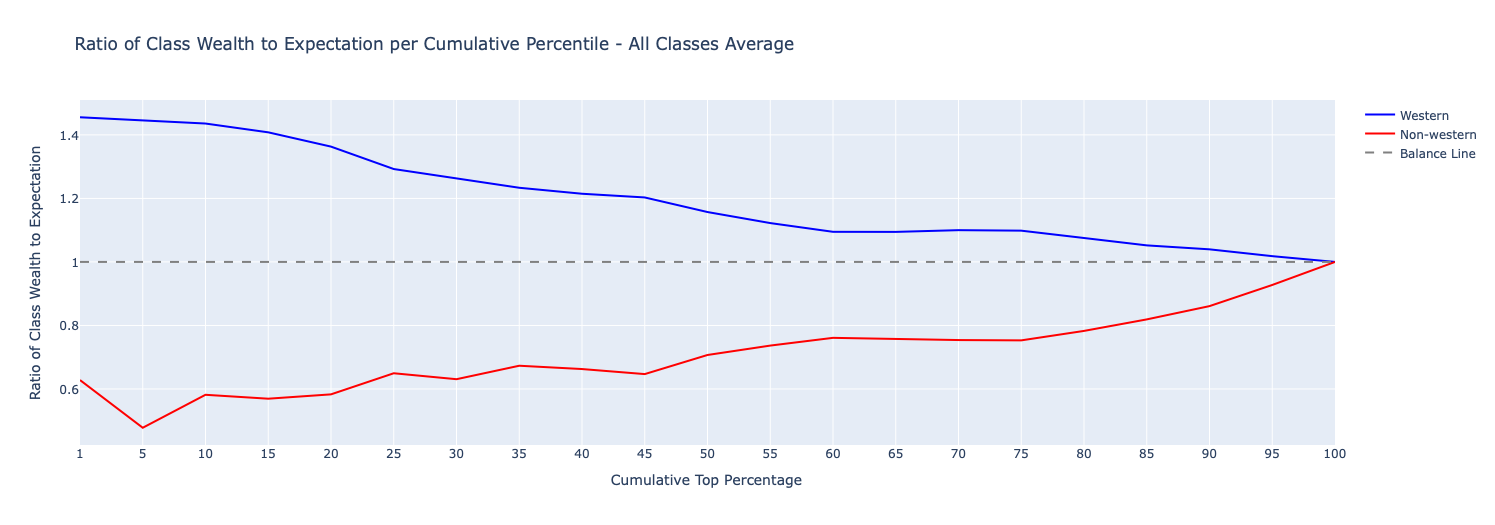
\includegraphics[clip,width=1.0\columnwidth]{Ratio of Class Wealth to Expectation per Cumulative Top Percentage - All Classes Average - Region}%
}

\subfloat[Ratio of Class Wealth to Expectation per Quantile - All Classes Average\label{fig:test2 - western}]{%
  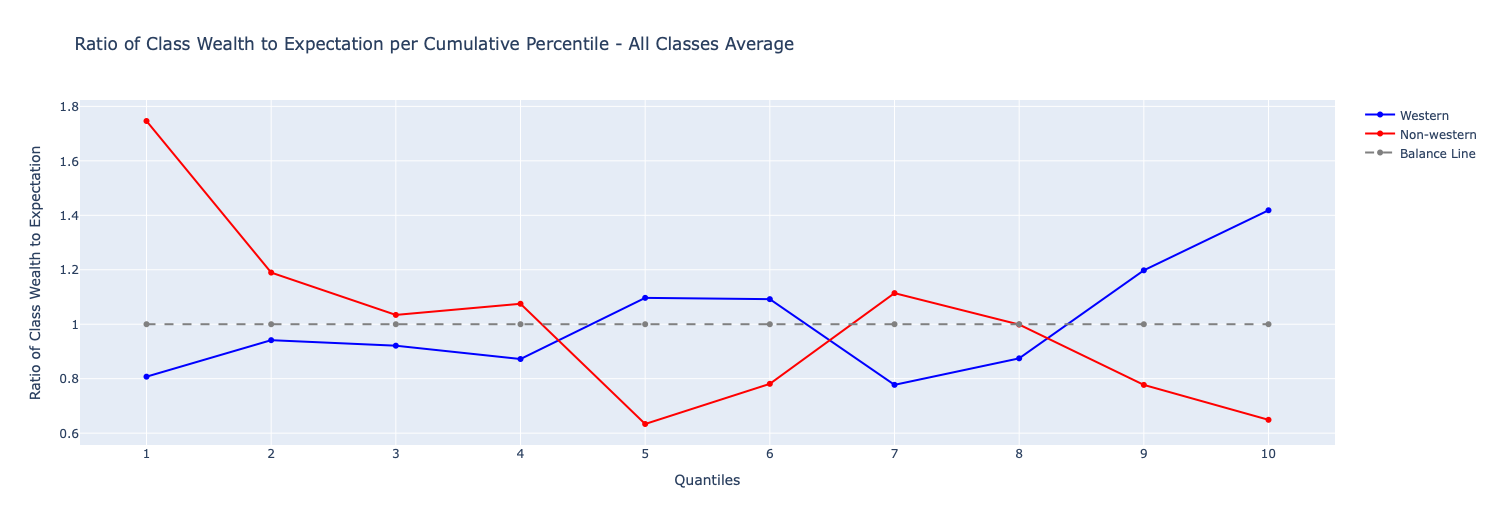
\includegraphics[clip,width=1.0\columnwidth]{Ratio of Class Wealth to Expectation per Quantile - All Classes Average - Gender - Region}%
}

\caption{Ratio of each regional wealth to expectation}\label{fig:western - ratio of regional wealth to expectation}

\end{figure}